\documentclass[conference]{IEEEtran}
\usepackage{cite,amsmath,amssymb,graphicx,booktabs,microtype,url}
\usepackage[hidelinks]{hyperref}
\usepackage[table]{xcolor}
\usepackage{tikz}
\usetikzlibrary{arrows.meta,positioning,calc,fit,backgrounds}
\newcommand{\todo}[1]{\textcolor{red}{[TODO: #1]}}
\begin{document}

\title{How Hackable Is Your Speech Quality Metric?\\A Corrected Protocol, a Benchmark, and What Patching Buys}

\author{\IEEEauthorblockN{Ali Alavi}
\IEEEauthorblockA{The Ohio State University\\
alavibajestan.1@osu.edu}}

\maketitle

\begin{abstract}
Speech quality predictors are increasingly used as rewards, so how easily they can be hacked is now a practical
question --- yet the field has no agreed way to measure it. We show the usual measurement is wrong in two ways,
then redo it. First, flagging a hack by comparing the attacked score with the \emph{raw input} conflates
the attack with how the predictor scores the processing chain itself; referenced correctly, to the zero-perturbation
codec round trip, measured hackability changes by up to a factor of four. Second, a single trained attacker is not
a measurement: retraining the same black-box GRPO attacker with different seeds moves its success rate between
0.00 and 0.38 against one fixed predictor, so a defence claim needs a worst case over several attackers. Applying
the corrected protocol to four predictors at an identical budget gives a wide and previously unreported spread:
NISQA is hacked on 90\% of utterances for $+0.95$ MOS, SSL-MOS on 21\%, DNSMOS on 14\% and UTMOS on 6\%, with
reconstruction offsets ranging from $-0.10$ to $+0.14$ MOS that make naive cross-metric comparisons
incommensurable. We then audit a closed attack--detect--patch loop with the protocol: it helps only in
the attack space it trains on, by less than attacker noise, a random-perturbation baseline with no RL and no
detector matches it, and the robustness costs up to 0.30 system SRCC out of domain, though enhancement models
post-trained against patched predictors do hack them far less (PESQ $-0.03$ versus $-0.23$). Code,
preregistration and all run outputs are released.
\end{abstract}

\begin{IEEEkeywords}
speech quality assessment, reward hacking, reinforcement learning, adversarial robustness, MOS prediction
\end{IEEEkeywords}

\section{Introduction}
Automatic mean-opinion-score (MOS) predictors are both the standard evaluation instrument for speech
generation~\cite{asonitis2026limits,huang2026attacking} and, increasingly, the \emph{reward} that trains
it~\cite{kumar2025rlhf,wang2026flowsegrpo,berdoz2026gspo}. Optimising a metric degrades what it was meant to
track~\cite{deoliveira2024pesqetarian,wang2026flowsegrpo}, and white-box attacks on UTMOS degrade speech
severely while its predicted MOS stays high~\cite{huang2026attacking}, so a generator could earn reward without
improving the audio. Those attacks only hold or lower the score of clean speech, whereas an RL-trained generator
sees only the score and is optimised to \emph{raise} it. Which predictor to reward with is a question practitioners must
answer, and the field answers it with intuition. There is no protocol for measuring how hackable a predictor is,
and no study that puts the predictors people actually use in front of the \emph{same} attacker, at the
\emph{same} perturbation strength, under the \emph{same} rule for what counts as a hack. Published attacks each
pick their own target, their own perturbation size and their own success criterion, so their numbers do not
share an axis: a predictor can look robust because it is, or merely because it was attacked more gently.

This matters well beyond MOS prediction as a research topic, because it is a property of every pipeline that
puts a learned quality model inside an optimisation loop. Speech enhancement is now routinely post-trained
against DNSMOS or NISQA rewards~\cite{wang2026flowsegrpo,wang2025sqase}, and whatever headroom a predictor
leaves is headroom the enhancer will find, so a deployed system can degrade on the very axis it reports
improving. Text-to-speech and voice conversion use the same predictors to select checkpoints, filter training
data and rank challenge submissions, so a hackable predictor quietly promotes the wrong system. In hearing aids
and other assistive processing the stakes are higher: quality and intelligibility predictors stand in for
listeners who cannot easily A/B test their own device, and a metric that an imperceptible perturbation lifts by
a full MOS point offers no assurance that a fitting which scores better sounds better. In each case the only
lever the practitioner has is which predictor to trust, and that choice is currently made blind.

This paper supplies the missing protocol and the missing comparison, and finds that the obvious way of
measuring is wrong twice over. A hack is a score that
rises \emph{because of the perturbation}, so the natural reference is the processing chain's own output, not the
raw input; using the raw input instead folds in how the predictor scores the codec itself, which we find varies
from $-0.10$ to $+0.14$ MOS across predictors and up to $+0.95$ MOS across defences. And because an attacker is
itself trained, one attacker is one sample: five attackers against a fixed predictor span success rates from
$0.00$ to $0.38$. Fixing both, we benchmark four widely used predictors at an identical budget and find a spread
of more than an order of magnitude, with the most hackable of them --- NISQA, commonly used as an RL reward ---
hacked on $90\%$ of utterances.

We then apply the protocol to the defence the diagnosis suggests: a closed attack--detect--patch loop in which a
black-box attacker finds hacks, a label-free rule detects them, and the predictor is patched on the resulting
pairs --- the speech counterpart of Adv-RM~\cite{bukharin2025advrm}, which we cite as the closest precedent but
cannot run across the modality gap. Correctly measured, it hardens only the space it trains on, by less than
attacker noise, and is matched by a baseline with no RL and no detector.

\noindent\textbf{Contributions.} (i) A measurement protocol for hackability --- reference the hack rule to the
processing chain's output, report the worst case over $k$ independently trained attackers --- and evidence that
both corrections change conclusions (Sec.~\ref{sec:results}). (ii) The first benchmark of common speech quality
predictors under one attack budget and one detector (Table~\ref{tab:bench}, Fig.~\ref{fig:results}a).
(iii) An audit of closed-loop patching with it: narrow hardening, negative transfer, a trivial baseline that
matches it, and the out-of-domain cost (Table~\ref{tab:e1}). (iv) Downstream evidence on reward hacking of a
small enhancement model (Table~\ref{tab:e3}). All data and models are public and every number is regenerated by
the released analysis scripts.

\section{Related work}
\label{sec:related}
\noindent\textbf{Quality metrics can be gamed.} Optimising a metric degrades true quality: the
PESQetarian~\cite{deoliveira2024pesqetarian} reaches 3.82 PESQ while listeners rate it poorly, FlowSE-GRPO % lint:ok (cited from prior work)
observes implausible DNSMOS gains under single-metric optimisation~\cite{wang2026flowsegrpo}, and composite
rewards are the usual remedy~\cite{berdoz2026gspo,wang2025sqase}. Asonitis et al.~\cite{asonitis2026limits} diagnose hacking --- the
optimised score rises as an independent panel falls --- but leave the predictor untouched.

\noindent\textbf{Attacking quality predictors.} Adversarial examples fool non-intrusive
predictors~\cite{lin2022robustness,ren2023eventtrojan}, and ``Attacking UTMOS''~\cite{huang2026attacking} attacks
codec latent spaces without proposing a defence. Lin et
al.~\cite{lin2022robustness} adversarially train DNSMOS once against waveform perturbations, without a hack
detector or a downstream generator; RRPO~\cite{wang2026rrpo} hardens a TTS reward model in one pass, as does
gradient-norm regularisation for image quality models~\cite{liu2024iqadefense}.

\noindent\textbf{Closing the loop.} Adv-RM~\cite{bukharin2025advrm} applies the same recipe to LLM reward models. Related ideas alternate policy and reward-model
updates~\cite{cheng2024apo,hong2025cooper,wolf2025iterated}, ensemble reward
models~\cite{coste2024ensembles,eisenstein2024helping}, harden agent benchmarks~\cite{zhong2026hackerfixer} or
post-train adversarially for music~\cite{wu2026gapt}. Our contribution is the measurement protocol, the benchmark it enables, and a
controlled audit of what the loop buys.

\begin{figure}[t]
\centering
\resizebox{\columnwidth}{!}{%
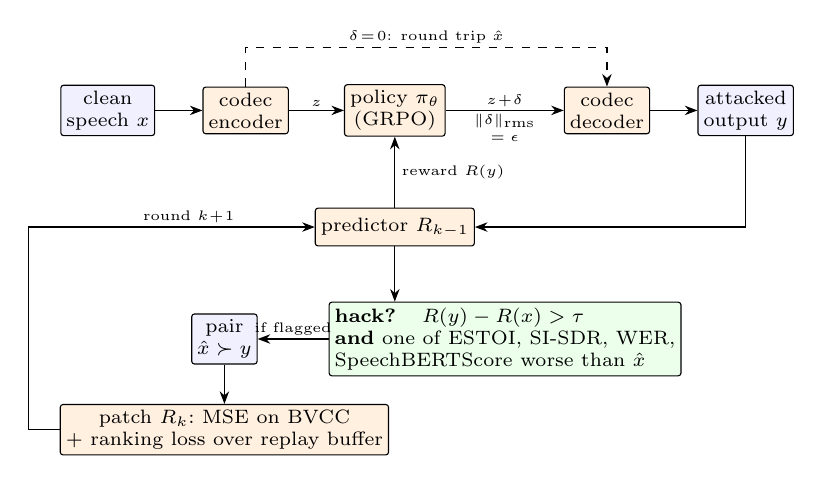
\begin{tikzpicture}[
  font=\scriptsize, >={Stealth[length=1.6mm]},
  box/.style={draw, rounded corners=1pt, align=center, inner sep=2pt, minimum height=4.8mm},
  sig/.style={box, fill=blue!6}, mod/.style={box, fill=orange!12},
  rule/.style={box, fill=green!8, align=left},
  lbl/.style={font=\tiny, inner sep=1.2pt}]

% ---- attack chain: gaps sized to the edge labels they carry ----
\node[sig] (x) {clean\\speech $x$};
\node[mod, right=6mm of x] (enc) {codec\\encoder};
\node[mod, right=7mm of enc] (pol) {policy $\pi_\theta$\\(GRPO)};
\node[mod, right=15mm of pol] (dec) {codec\\decoder};
\node[sig, right=6mm of dec] (y) {attacked\\output $y$};

\draw[->] (x) -- (enc);
\draw[->] (enc) -- node[lbl, above] {$z$} (pol);
\draw[->] (pol) -- node[lbl, above] {$z\!+\!\delta$}
                   node[lbl, below, align=center] {$\|\delta\|_{\mathrm{rms}}$\\$=\epsilon$} (dec);
\draw[->] (dec) -- (y);

% ---- zero-perturbation bypass: the corrected reference, routed above the row ----
\draw[->, dashed] (enc.north) -- ++(0,5mm)
  -- node[lbl, above] {$\delta\!=\!0$: round trip $\hat{x}$} ($(dec.north)+(0,5mm)$) -- (dec.north);

% ---- scoring ----
\node[mod, below=9mm of pol] (R) {predictor $R_{k-1}$};
\draw[->] (y) |- (R);
\draw[->] (R) -- node[lbl, right=0.4mm] {reward $R(y)$} (pol);

% ---- detector ----
\node[rule, below=7mm of R, xshift=14mm] (det)
  {\textbf{hack?} \; $R(y)-R(x) > \tau$\\ \textbf{and} one of ESTOI, SI-SDR, WER,\\ SpeechBERTScore worse than $\hat{x}$};
\draw[->] (R.south) -- (det.north -| R.south);

\node[sig, left=9mm of det] (pair) {pair\\$\hat{x} \succ y$};
\draw[->] (det.west) -- node[lbl, above] {if flagged} (pair.east);

\node[mod, below=5mm of pair] (patch) {patch $R_k$:\ MSE on BVCC\\$+$ ranking loss over replay buffer};
\draw[->] (pair) -- (patch);
\draw[->] (patch.west) -- ++(-4mm,0) |- node[lbl, pos=0.78, above] {round $k\!+\!1$} (R.west);
\end{tikzpicture}}
\caption{The attack--detect--patch loop. A GRPO policy perturbs codec latents at a fixed budget; an output is
flagged only if the score rises \emph{and} an independent panel degrades relative to the zero-perturbation round
trip $\hat{x}$ (dashed); flagged pairs patch the predictor, and the next round retrains the attacker.}
\label{fig:method}
\end{figure}

\section{Method}
\label{sec:method}
Let $R$ be a mean-opinion-score (MOS) predictor mapping a waveform to a scalar. The loop (Fig.~\ref{fig:method}) has three parts.

\noindent\textbf{Attacker.}
Speech $x$ is encoded to a continuous latent $z=\mathrm{Enc}(x)$ by a frozen neural codec~\cite{defossez2023encodec}. A policy
$\pi_\theta$ proposes an action $a\sim\mathcal{N}(\mu_\theta(z),\sigma^2)$ in per-channel standardised latent
units; the perturbation $\delta=\mathrm{expand}(a)$ is rescaled to a fixed root-mean-square budget $\epsilon$,
and the attacked signal is $y=\mathrm{Dec}(z+\delta\odot s_z)$ with $s_z$ the per-channel latent standard
deviation. The policy is trained with GRPO~\cite{shao2024grpo}: for each utterance we draw $G$ actions, score them with the frozen
target predictor, and use group-normalised advantages $A_{ij}=(r_{ij}-\bar r_i)/(\mathrm{std}_j r_i+\eta)$ with
$r=R(y)$, optimised with a clipped surrogate. The action is time-invariant (one $C$-dimensional offset per
utterance), which keeps the policy-gradient variance tractable: a frame-rate action space did not learn at any
budget we tried. The attacker needs only forward scores, so any predictor can be a target.

\noindent\textbf{Label-free hack detection.}
An attacked output $y$ is flagged as a \emph{hack} when both rules hold:
(i) \emph{ceiling rule} --- $R(y)-R(x)>\tau$, i.e. the predictor scores the attacked signal above the
unattacked input by more than $\tau$ MOS; and
(ii) \emph{panel rule} --- at least one independent measure is worse for $y$ than for the codec round trip
$\hat{x}=\mathrm{Dec}(z)$ by more than a per-measure margin: ESTOI, SI-SDR, SpeechBERTScore~\cite{saeki2024speechbertscore} (all against $x$),
or the word error rate of Whisper transcripts of $y$ against those of $x$.
Comparing the panel against $\hat{x}$ rather than $x$ is what isolates the effect of the perturbation from the
codec's own round-trip loss. No human labels are used. The fraction of utterances an attacker gets flagged this
way is its \emph{attack success rate} (ASR), our measure of hackability.

\noindent\textbf{Patch.}
Every flagged hack contributes one preference pair $\hat{x}\succ y$. The predictor is fine-tuned on the sum of
the original regression loss on the human-labelled training set and a margin ranking loss
$\max(0, m-(R(\hat{x})-R(y)))$ over a replay buffer that keeps the hacks of all previous rounds. Using $\hat{x}$
rather than $x$ as the preferred side prevents the predictor from solving the task with a ``codec artefact''
shortcut; an exploratory ablation ($n\!=\!1$) confirms it, with in-loop ASR reaching $0.010$ by round~3 against
$0.172$ when $x$ is used. Attack, detection and patching are repeated for $K$ rounds, giving $R_1,\dots,R_K$.

\noindent\textbf{Multi-space variant.}
The same loop can draw its pairs from several attack spaces at once. In addition to the codec latent space above
we use (i) a second codec (DAC~\cite{kumar2023dac}, quantised latent) and (ii) white-box waveform PGD that
maximises $R$ under $\|\delta\|_\infty\le 0.002$. All flagged hacks share one buffer.

\section{Experimental setup}
\label{sec:setup}
\noindent\textbf{Predictor and data.} $R_0$ is SSL-MOS~\cite{cooper2022generalization}: a wav2vec\,2.0 base % lint:ok
encoder with mean pooling and a linear head, trained with MSE on the BVCC training split (4\,974 utterances) % lint:ok
for 8\,000 steps (AdamW, $2\!\times\!10^{-5}$ encoder / $10^{-3}$ head, batch 8, 6\,s crops), selecting the best % lint:ok
validation-MSE checkpoint. Human agreement is evaluated on 13 test sets: BVCC test, the VoiceMOS'22
out-of-domain set, three NISQA sets, SOMOS, TMHINT-QI, four VoiceMOS'23 tracks and the URGENT'24/'25 % lint:ok
quality-assessment sets.

\noindent\textbf{Attacker and detector.} The attack space is the continuous EnCodec-24\,kHz latent % lint:ok
(128 channels at 75\,Hz); the policy is a four-layer 1-D convolutional network (256 hidden units) with a % lint:ok
per-channel learned $\sigma$, trained for 2\,000 GRPO steps ($G=8$, batch 8, 3\,s crops, lr $10^{-3}$, % lint:ok
clip 0.2, two inner epochs). The budget $\epsilon=0.5$ was selected on the validation split alone
(Sec.~\ref{sec:results}). The detector uses $\tau=0.3$ MOS with margins of 0.02 ESTOI, 1\,dB SI-SDR, 0.02
SpeechBERTScore and any WER increase (Whisper-small; HuBERT-base layer 8). % lint:ok

\noindent\textbf{Patching and baselines.} Each round fine-tunes for 1\,500 steps with equal MSE and ranking % lint:ok
batches (margin $m=0.5$, weight 1) and $K=3$ rounds. Three defences receive the identical 4\,500-step budget and % lint:ok
loss, differing in where the rejected side comes from: Gaussian noise pairs (SNR 5--30\,dB), waveform-PGD % lint:ok
pairs, and random latent perturbations at the same budget $\epsilon$ (no RL, no detector). PGD uses
$\|\delta\|_\infty\!\le\!0.002$ with 50 steps at evaluation but 10 steps inside the multi-space loop and 5 in the % lint:ok
PGD-pair baseline, so those defences meet a weaker attacker than they are tested against; training is
step-matched but not pair-matched (replay buffer 5.8k to 8.9k pairs against 19.9k random pairs, % lint:ok
favouring the baseline).

\noindent\textbf{Downstream (E3).} A 2.6\,M-parameter STFT mask enhancer is pre-trained on VoiceBank-DEMAND and % lint:ok
post-trained with GRPO for 2\,500 steps, the policy adding per-frame offsets on 32 ERB bands with no KL % lint:ok
penalty, so only the reward model limits hacking. Evaluation uses the 824-utterance test set. % lint:ok

\noindent\textbf{Protocol.} Seeds, primary metrics and decision rules for E1--E3 were preregistered before any
test-label contact, with one amendment (attack action space and the $\epsilon$ rule) made on validation evidence
before the main runs; the multi-space variant and the ablations are exploratory additions, and the corrected
ceiling reference is a post-hoc re-analysis of stored per-utterance outputs. Results are reported over $n$ seeds as mean\,$\pm$\,standard deviation.


\begin{figure*}[t]
\centering
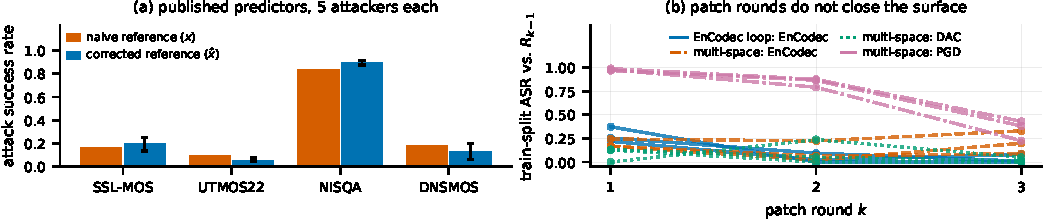
\includegraphics[width=\textwidth]{figs/results.pdf}
\caption{(a) Benchmark of four common predictors at one budget under the naive ($x$) and corrected ($\hat{x}$)
ceiling references; error bars span the five independently trained attackers. The reference choice moves DNSMOS
and NISQA in \emph{opposite} directions. (b) In-loop attack success rate (BVCC train, corrected reference) of
the round-$k$ attacker against the predictor patched in round $k\!-\!1$, one line per seed: the single-space
loop converges in its own space, while under multi-space training DAC and PGD fall and the EnCodec attacker
stays flat (mean change $+0.01$).}
\label{fig:results}
\end{figure*}

\section{Results}
\label{sec:results}

\begin{table}[t]
\centering
\caption{\textbf{Hackability of common predictors} at one budget ($\epsilon\!=\!0.5$, EnCodec latents), five
independently trained attackers each, 500 BVCC-test utterances; ``worst'' is the largest of the five.}
\label{tab:bench}
\footnotesize
\setlength{\tabcolsep}{3pt}
% generated by analysis/paper_assets.py
\begin{tabular}{l c c c c}
\toprule
Predictor & offset & mean ASR & worst ASR & mean gain \\
\midrule
SSL-MOS (BVCC) & -0.10 & 0.205 & 0.252 & +0.191 \\
UTMOS22 & -0.07 & 0.057 & 0.076 & +0.144 \\
NISQA & +0.14 & 0.896 & 0.916 & +0.954 \\
DNSMOS OVRL & +0.02 & 0.136 & 0.200 & +0.124 \\
\bottomrule
\end{tabular}

\end{table}

\noindent\textbf{The reference of the hack rule changes the answer.} A defence or a predictor that scores
codec-processed audio differently from raw audio shifts every raw-input-referenced measurement with it. That
offset is not negligible and not constant: $-0.10$ (SSL-MOS), $-0.07$ (UTMOS), $+0.02$ (DNSMOS) and $+0.14$
(NISQA) across predictors (Table~\ref{tab:bench}), and up to $+0.95$ across the defences of
Table~\ref{tab:e1}. The consequences are concrete: under the naive reference DNSMOS looks \emph{more}
hackable than it is ($0.183$ vs $0.136$), NISQA \emph{less} ($0.839$ vs $0.896$), and the multi-space defence
below flips from apparently catastrophic ($0.306$) to among the most robust ($0.082$). We reference every result to the
codec round trip $\hat{x}$.

\noindent\textbf{One attacker is not a measurement.} Retraining the attacker with different seeds against one
fixed predictor gives ASR from $0.000$ to $0.261$ on $R_0$ and $0.000$ to $0.382$ on $R_3$ (sd $0.130$ and
$0.180$) --- as large as every defence effect we measure. Between \emph{predictors}, by contrast, the spread is
small relative to the differences (NISQA $0.876$--$0.916$ against UTMOS $0.042$--$0.076$), so the benchmark
ranking is solid where defence comparisons are not. We therefore report the worst of five attackers.

\noindent\textbf{Common predictors differ by more than an order of magnitude (Table~\ref{tab:bench}).} At an
identical budget, NISQA is hacked on $89.6\%$ of utterances for a mean gain of $+0.954$ MOS, SSL-MOS on
$20.5\%$, DNSMOS OVRL on $13.6\%$ and UTMOS on $5.7\%$; worst-case rates are $0.916$, $0.252$, $0.200$ and
$0.076$. As NISQA and DNSMOS are routinely used as RL rewards, the choice of reward is a
first-order robustness decision, and the ranking is not predictable from in-domain accuracy.

\begin{table*}[t]
\centering
\caption{\textbf{Auditing the loop.} Corrected-reference ASR per attack space (fresh attacker, BVCC test) and
agreement with human MOS (BVCC system SRCC; out-of-domain mean over 12 sets). Mean$\pm$sd over 3 seeds.}
\label{tab:e1}
\footnotesize
\setlength{\tabcolsep}{3.5pt}
% generated by analysis/paper_assets.py
\begin{tabular}{l c c c c c c}
\toprule
& offset & \multicolumn{3}{c}{ASR by attack space} & \multicolumn{2}{c}{human agreement} \\
\cmidrule(lr){3-5}\cmidrule(lr){6-7}
Predictor & $R(\hat{x})\!-\!R(x)$ & EnCodec & DAC & PGD & BVCC & OOD \\
\midrule
$R_0$ (no defense) & -0.09$\pm$0.02 & 0.226$\pm$0.205 & 0.065$\pm$0.113 & 0.999$\pm$0.002 & 0.922$\pm$0.004 & 0.731$\pm$0.006 \\
$R_1$ & -0.06$\pm$0.03 & 0.050$\pm$0.048 & 0.161$\pm$0.033 & 1.000$\pm$0.001 & 0.911$\pm$0.009 & 0.690$\pm$0.014 \\
$R_2$ & 0.00$\pm$0.07 & 0.017$\pm$0.006 & 0.141$\pm$0.025 & 1.000$\pm$0.000 & 0.918$\pm$0.003 & 0.682$\pm$0.008 \\
$R_3$ (EnCodec loop) & -0.27$\pm$0.25 & 0.137$\pm$0.179 & 0.127$\pm$0.031 & 1.000$\pm$0.000 & 0.920$\pm$0.001 & 0.637$\pm$0.046 \\
$R_3^{\mathrm{multi}}$ (multi-space) & 0.95$\pm$0.16 & 0.082$\pm$0.107 & 0.016$\pm$0.026 & 0.841$\pm$0.089 & 0.914$\pm$0.003 & 0.552$\pm$0.015 \\
noise pairs & -0.09$\pm$0.01 & 0.270$\pm$0.107 & 0.230$\pm$0.028 & 1.000$\pm$0.000 & 0.917$\pm$0.004 & 0.722$\pm$0.013 \\
PGD pairs & -0.08$\pm$0.02 & 0.223$\pm$0.057 & 0.225$\pm$0.044 & 0.969$\pm$0.025 & 0.909$\pm$0.001 & 0.635$\pm$0.009 \\
random-latent pairs & -0.03$\pm$0.03 & 0.019$\pm$0.016 & 0.200$\pm$0.053 & 1.000$\pm$0.000 & 0.922$\pm$0.004 & 0.696$\pm$0.010 \\
\bottomrule
\end{tabular}

\end{table*}

\noindent\textbf{Patching hardens narrowly, and a trivial baseline matches it (Table~\ref{tab:e1}).} Three
rounds against the EnCodec attacker cut ASR from $0.226\!\pm\!0.205$ ($R_0$) to $0.050$ ($R_1$) and $0.017$
($R_2$), and the replayed round-1 attacker never succeeds. The effect is not monotone --- $K\!=\!3$ was
preregistered rather than selected, and $R_2$ dominates $R_3$ on both axes --- and the $R_0\!\to\!R_3$ difference
does not hold its sign across seeds ($-0.073$, $-0.039$, $+0.379$), so our preregistered H1, which passes under
the naive reference, fails under the corrected one. Pairs from \emph{random} latent perturbations at the same
budget, with no RL and no detector, give the lowest in-space ASR of any defence ($0.019\!\pm\!0.016$). Since the
patch margin ($m\!=\!0.5$) exceeds the detection threshold ($\tau\!=\!0.3$) we swept $\tau\in[0.1,1.0]$: the
ordering is unchanged, though $R_3$ alone keeps a tail of large hacks (ASR $0.045$ at $\tau\!=\!1.0$;
90th-percentile score gap $0.651$ vs $0.359$ for $R_0$).

\begin{table}[!tb]
\centering
\caption{\textbf{Downstream GRPO enhancement.} Change against the supervised pre-trained enhancer on
VoiceBank-DEMAND test, per reward predictor. Mean$\pm$sd over 3 seeds ($R_2$: one seed).}
\label{tab:e3}
\footnotesize
\setlength{\tabcolsep}{3pt}
% generated by analysis/paper_assets.py
\begin{tabular}{l c c c}
\toprule
Measure & $R_0$ & $R_3$ & random-latent pairs \\
\midrule
$\Delta$ own reward & 0.263$\pm$0.010 & 0.269$\pm$0.028 & 0.334$\pm$0.051 \\
$\Delta$PESQ & -0.226$\pm$0.170 & -0.034$\pm$0.126 & 0.019$\pm$0.050 \\
$\Delta$ESTOI & -0.057$\pm$0.010 & -0.038$\pm$0.013 & -0.043$\pm$0.006 \\
$\Delta$SI-SDR (dB) & -6.1$\pm$1.4 & -5.8$\pm$1.4 & -5.7$\pm$0.6 \\
$\Delta$DNSMOS & -0.075$\pm$0.031 & -0.076$\pm$0.056 & -0.075$\pm$0.043 \\
$\Delta$NISQA & 0.335$\pm$0.186 & 0.300$\pm$0.072 & 0.468$\pm$0.059 \\
$\Delta$UTMOS & 0.018$\pm$0.006 & 0.057$\pm$0.030 & 0.076$\pm$0.011 \\
\bottomrule
\end{tabular}

\end{table}

\noindent\textbf{No transfer, and one real trade.} Against an unseen DAC attacker the EnCodec-patched predictors
are \emph{worse} than undefended ($0.065$ to between $0.13$ and $0.16$), and white-box PGD succeeds on nearly
every utterance for every EnCodec-trained defence. Only multi-space training changes this: it resists DAC
($0.016$) and is the one predictor PGD does not fully break ($0.841\!\pm\!0.089$), paying with the $+0.95$ MOS
reconstruction offset and the largest loss of human agreement. In-loop, DAC and PGD fall round by round while the
EnCodec attacker stays flat (Fig.~\ref{fig:results}b).

\noindent\textbf{Fidelity: ranking holds in domain, calibration and out-of-domain agreement do not.} The patched
predictors keep their BVCC system ranking ($R_3$ $0.920$ vs $R_0$ $0.922$, meeting the preregistered $-0.02$
margin) but utterance MSE rises $0.234\!\pm\!0.011\to0.272\!\pm\!0.022$, a calibration loss that matters for a
reward model. Out of domain the mean system SRCC falls from $0.731$ to $0.690$, $0.682$ and $0.637$ over rounds
one to three and to $0.552$ for $R_3^{\mathrm{multi}}$, worst on noisy speech (TMHINT-QI, where the $R_0$ and
$R_3$ bootstrap intervals do not overlap; TMHINT-QI and VoiceMOS'23 track~3 share a condition grid and are not
independent). A predictor taught that perturbed audio is bad seems to generalise that to genuinely noisy audio.


\noindent\textbf{Downstream, patched predictors are safer rewards --- and so is the baseline
(Table~\ref{tab:e3}).} Against $R_0$ the enhancer shows the textbook hack: reward $+0.263$ while PESQ falls
$-0.226$, ESTOI $-0.057$ and SI-SDR $-6.1$\,dB. Against $R_3$ the reward rises as much ($+0.269$) with PESQ
intact ($-0.034$), and $R_2$ behaves the same ($+0.378$, $-0.034$), so this is a property of patching rather than
of one round; the random-pair baseline again matches it ($+0.019$). Preregistered H3 is \emph{not} supported (2.33 degraded measures for
both rewards): NISQA and UTMOS \emph{rise} and DNSMOS falls under every reward, so none detects this hack, while
speaker similarity and WER barely move. $R_3$ scores the $R_0$-hacked enhancer $2.77$ against $3.72$ for the pre-trained model
--- flagging a generator that hacked a \emph{different} predictor, though not the one that hacked itself
($3.99$), and without a loudness-matched control we cannot separate this from ``scores degraded audio lower''.

\section{Conclusion}
How hackable a speech quality predictor is depends on two measurement choices the field has not standardised:
whether the hack rule is referenced to the processing chain's own output, and whether hackability is reported for
one attacker or for the worst of several. Corrected on both, common predictors differ by more than an order of
magnitude at the same budget --- NISQA $0.90$ against UTMOS $0.06$ --- so the choice of reward model is itself a
robustness decision. Patching a predictor on its own hacks hardens only the space it trains
on and is matched by a random-perturbation baseline.

Two caveats bound these conclusions. Our attacker is black-box and mild --- against SSL-MOS its flagged hacks
move ESTOI by only $-0.023$ and SI-SDR by $-1.034$\,dB, and two independent judges call them perceptually
marginal (UTMOS $-0.004$, DNSMOS OVRL $-0.048$), against $+0.802$ UTMOS for PGD --- and we ran no listening
test, so the benchmark ranks predictors against \emph{this} attack family only. The detector is also not fully
independent: two panel measures are neural and attackable in principle, and for waveform attacks its reference
is the input itself, so ASR is not comparable across attack families. The patch study uses $n=3$ predictor seeds
and one predictor family. Code and preregistration are released (46 A100-hours).

\bibliographystyle{IEEEtran}
\bibliography{refs}
\end{document}
